% !TEX root = ../main.tex

\begin{frame}{Audio Mixer Controls: Levels}
	\begin{columns}[T,onlytextwidth]
		\column{0.6\textwidth}
		\begin{figure} 
			\centering
			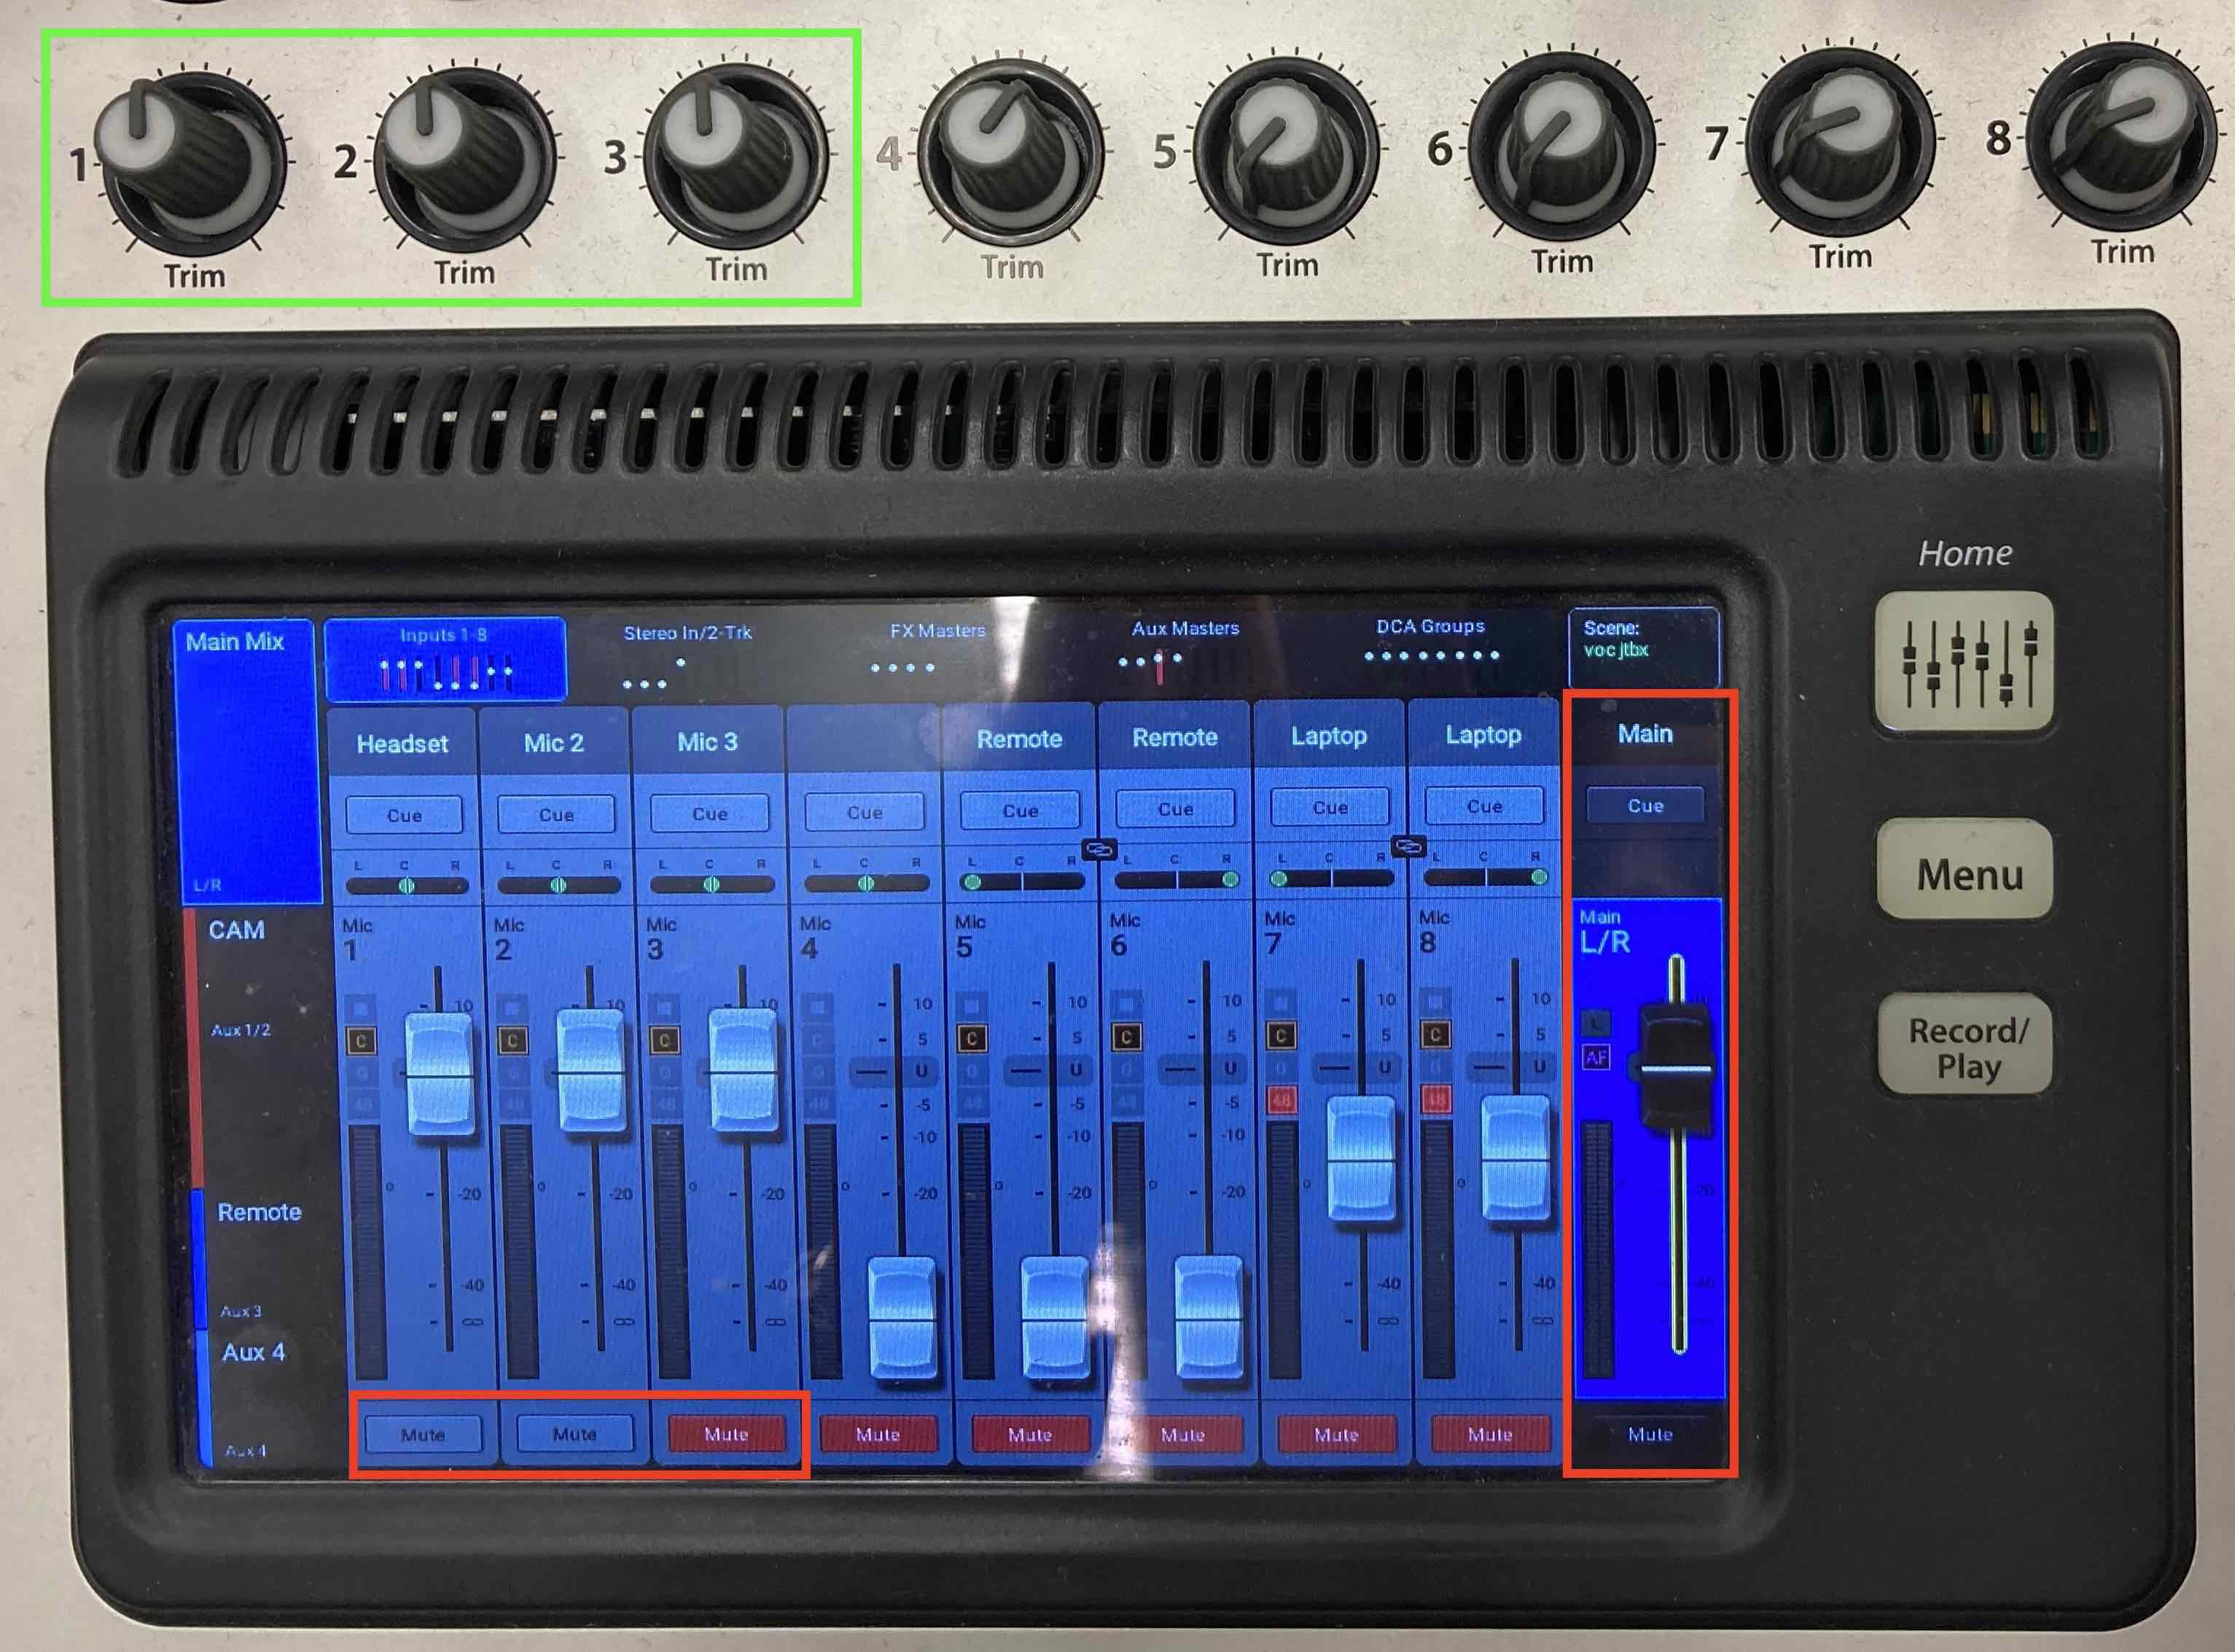
\includegraphics[width=0.9\textwidth]{images/touchmix-main-controls.jpg}
			\caption{Touchmix Main Controls}
		\end{figure}
		\column{0.4\textwidth}
		\begin{itemize}
			\item Mute unused microphones (bottom row)
			\item Adjust hall loudness with rightmost fader
			\item Adjust individual microphone level with fader or reduce "trim" knob when it's clipping
			\item Please keep microphones un-muted during applause
		\end{itemize}
	\end{columns}
\end{frame}

\begin{frame}{Audio Mixer Controls: Second Page}
	\begin{columns}[T,onlytextwidth]
		\column{0.6\textwidth}
		\begin{figure} 
			\centering
			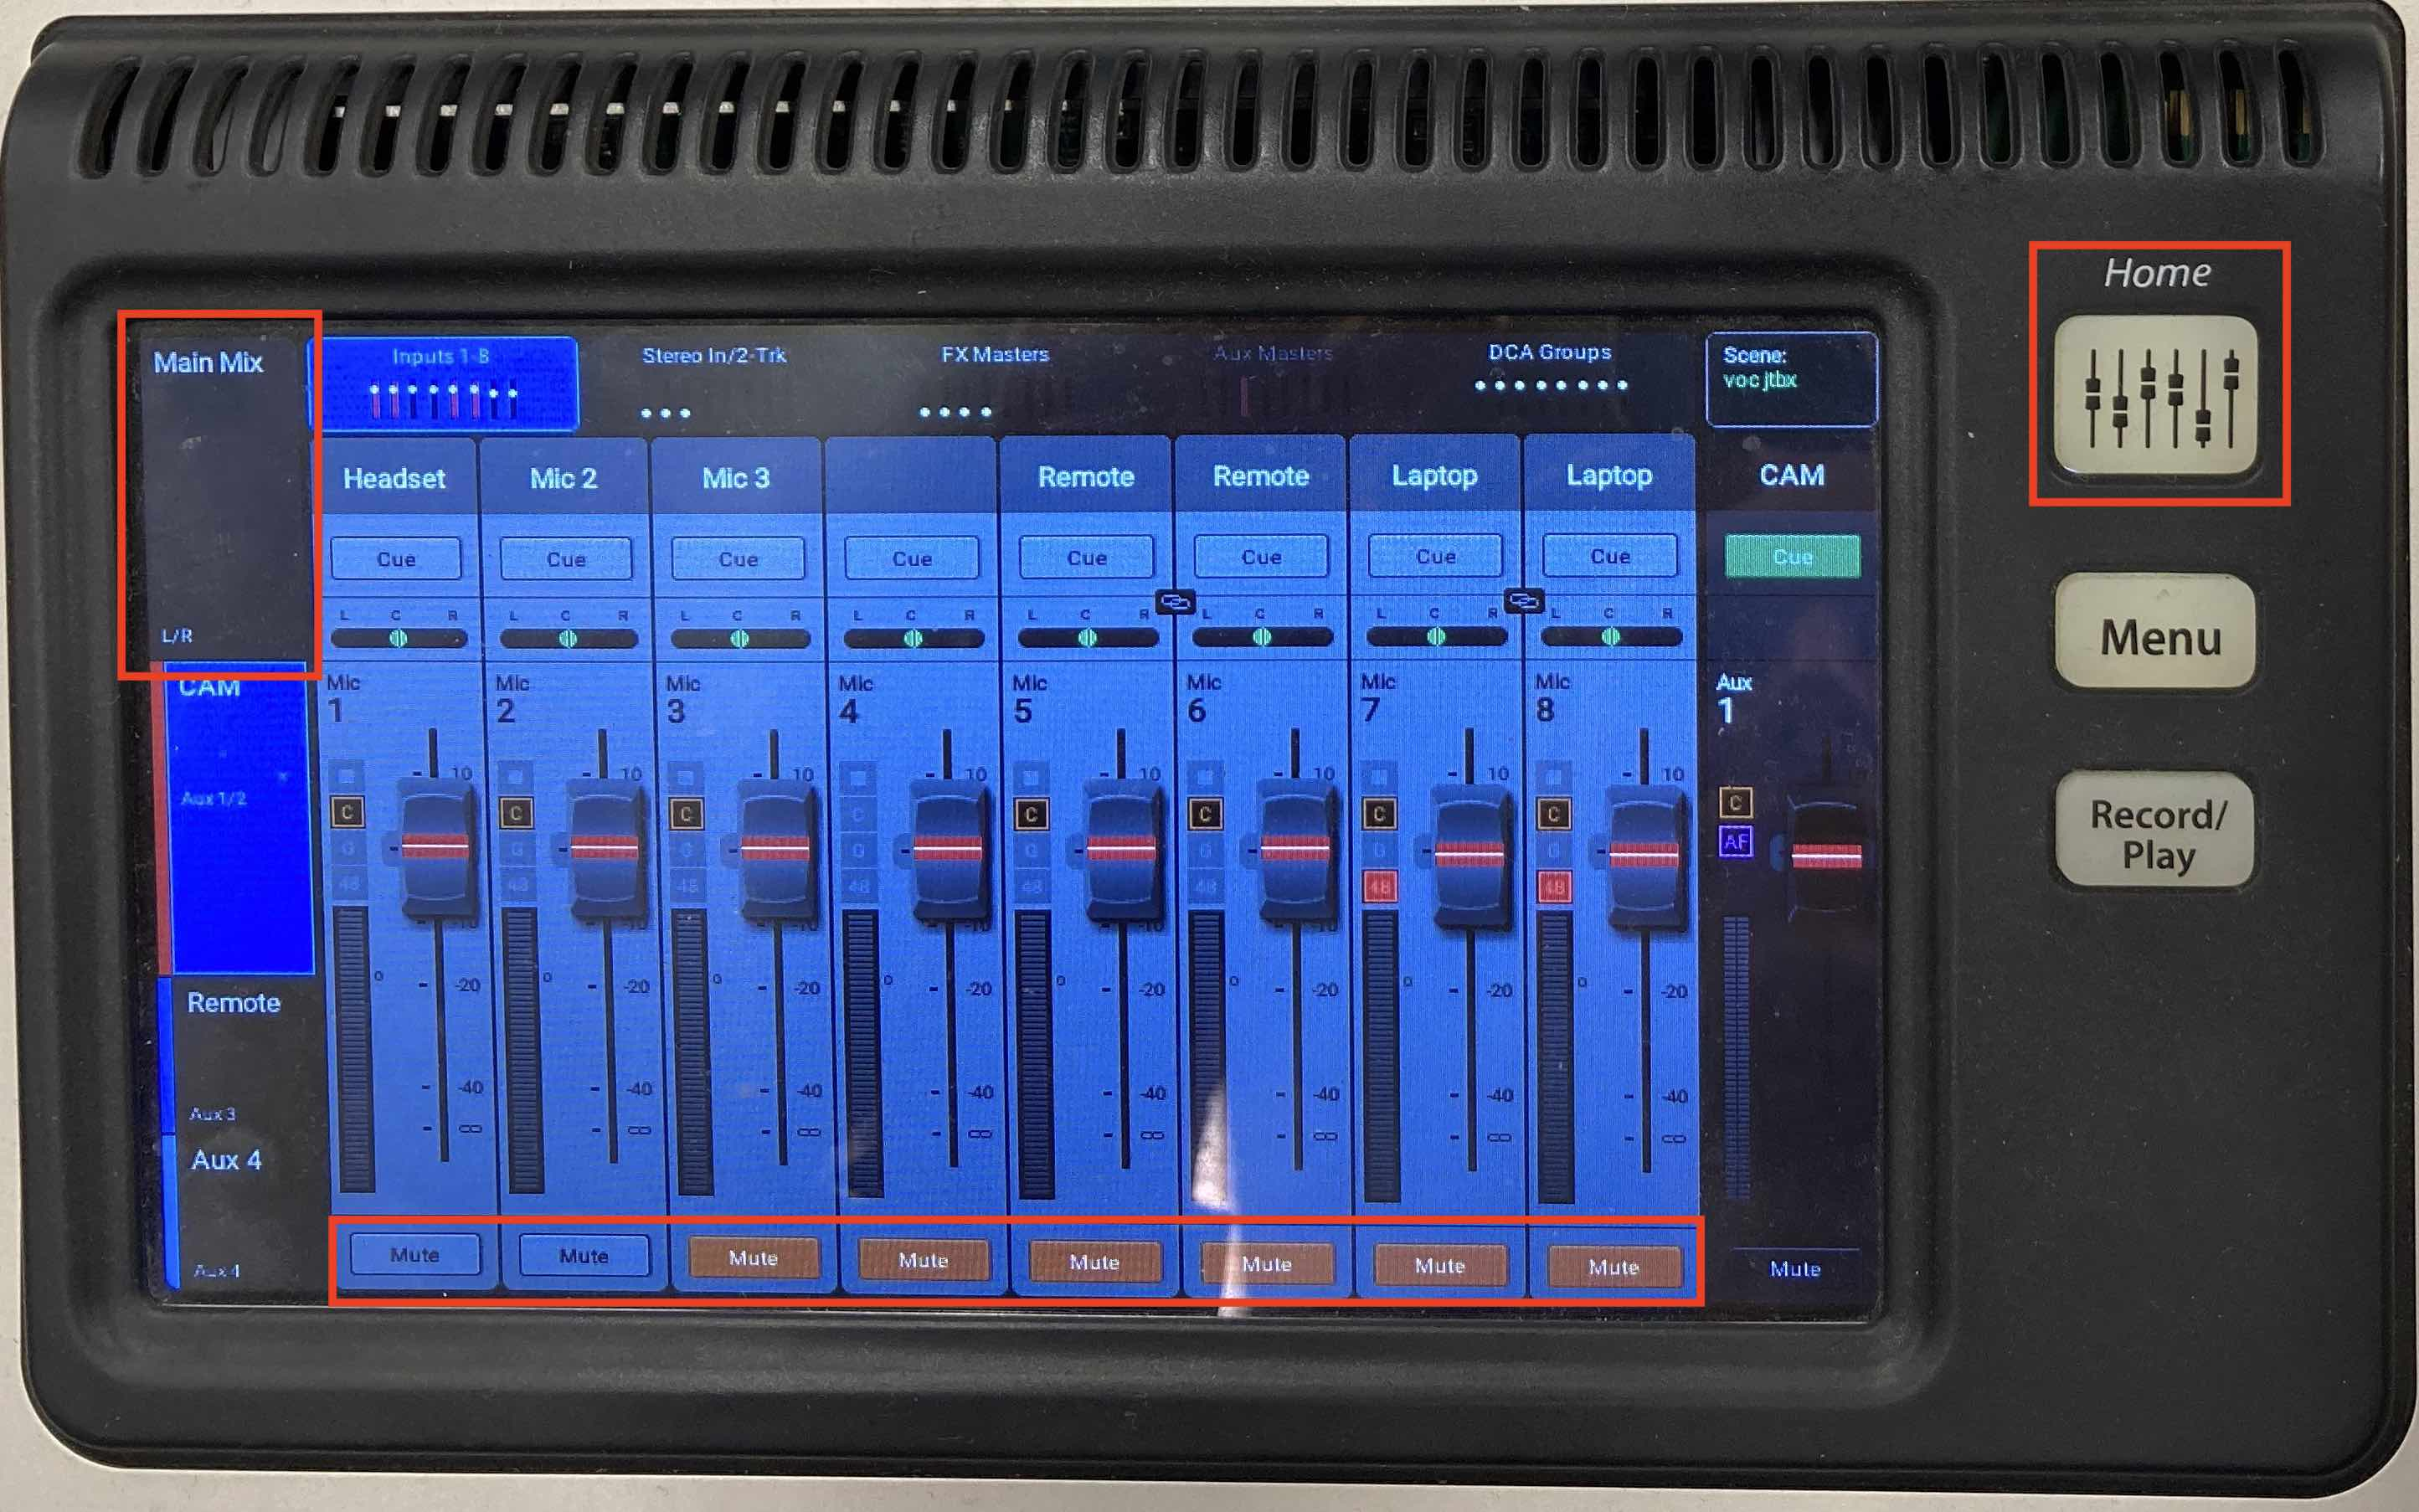
\includegraphics[width=0.9\textwidth]{images/touchmix-cam-controls.jpeg}
			\caption{Touchmix Second Page}
		\end{figure}
		\column{0.4\textwidth}
		\begin{itemize}
			\item If mute buttons are yellow, go back to "Main Mix" page
			\item If anything else is shown, just press "Home" button
		\end{itemize}
	\end{columns}
\end{frame}

\begin{frame}{Audio Mixer Controls: Headphones}
	\begin{columns}[T,onlytextwidth]
		\column{0.6\textwidth}
		\begin{figure} 
			\centering
			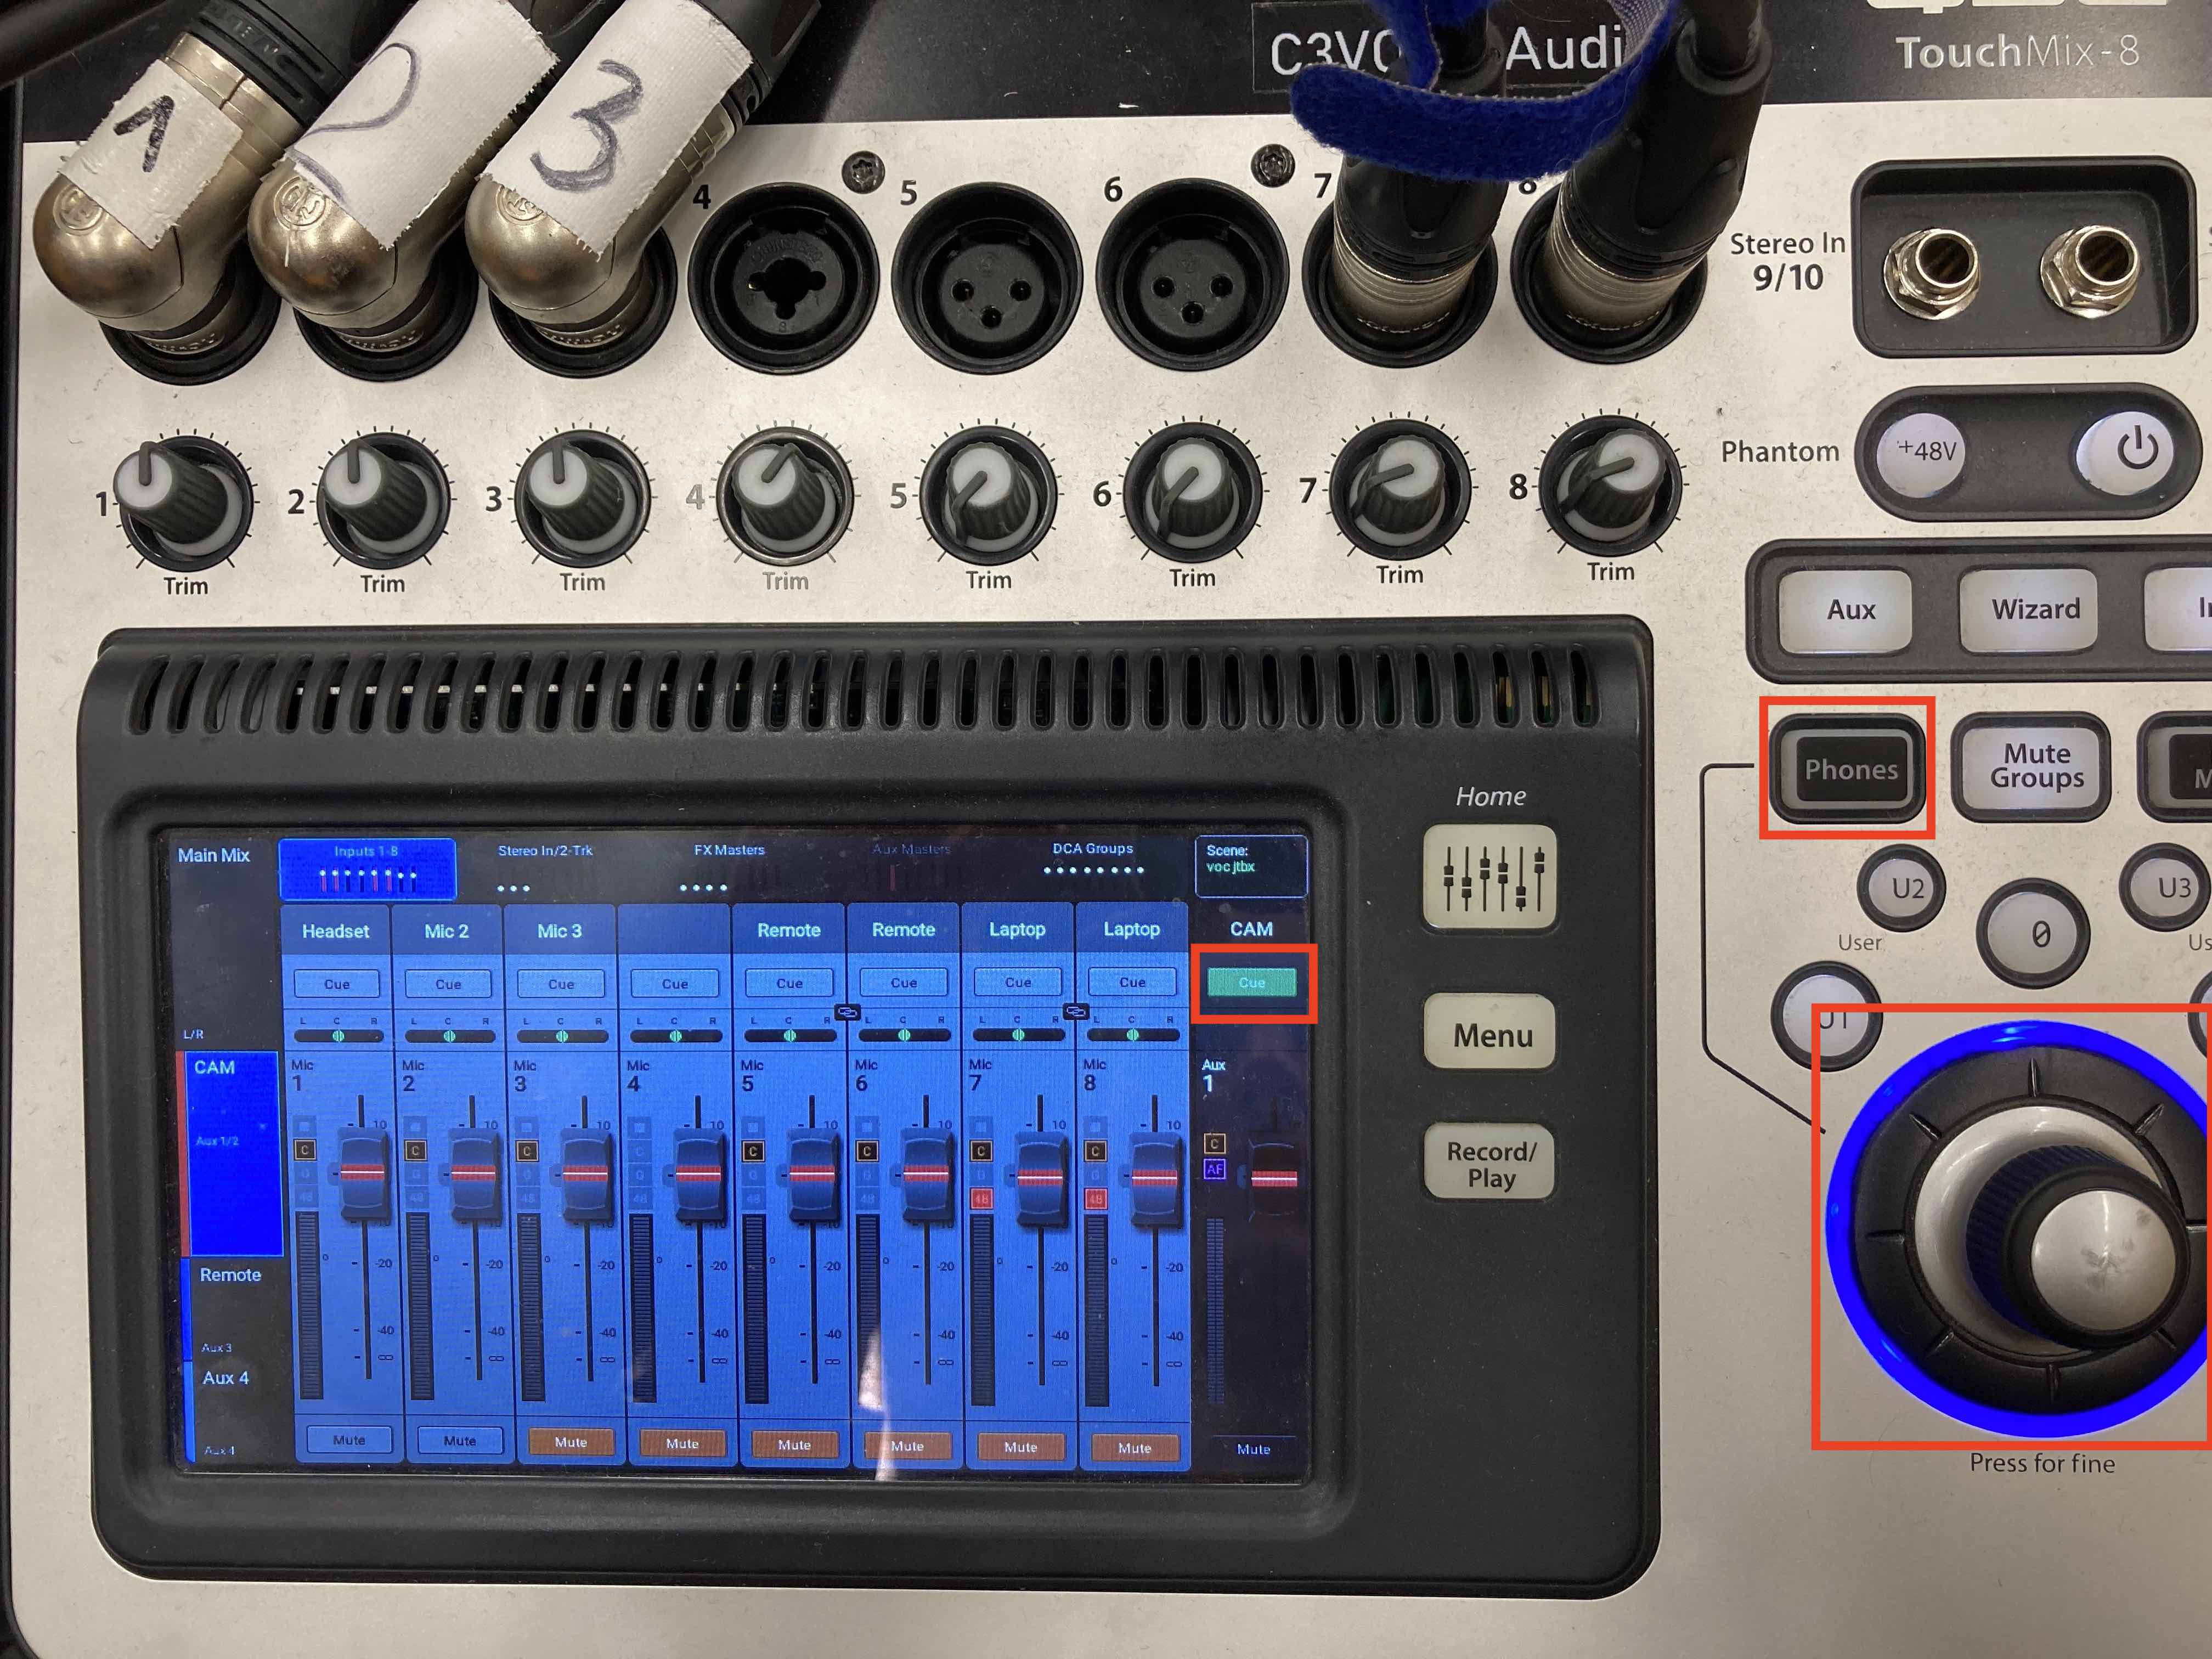
\includegraphics[width=0.9\textwidth]{images/touchmix-cam-headphones.jpg}
			\caption{Touchmix Headphones}
		\end{figure}
		\column{0.4\textwidth}
		\begin{itemize}
			\item Press "Phones" to adjust headphone loudness
			\item "Cue" on Camera/ Recoding mix must be selected
			\item Rotary knob can be used to adjust selected parameter (headphone level, channel level, etc.)
		\end{itemize}
	\end{columns}
\end{frame}
